% Options for packages loaded elsewhere
\PassOptionsToPackage{unicode}{hyperref}
\PassOptionsToPackage{hyphens}{url}
%
\documentclass[
  ignorenonframetext,
]{beamer}
\usepackage{pgfpages}
\setbeamertemplate{caption}[numbered]
\setbeamertemplate{caption label separator}{: }
\setbeamercolor{caption name}{fg=normal text.fg}
\beamertemplatenavigationsymbolsempty
% Prevent slide breaks in the middle of a paragraph
\widowpenalties 1 10000
\raggedbottom
\setbeamertemplate{part page}{
  \centering
  \begin{beamercolorbox}[sep=16pt,center]{part title}
    \usebeamerfont{part title}\insertpart\par
  \end{beamercolorbox}
}
\setbeamertemplate{section page}{
  \centering
  \begin{beamercolorbox}[sep=12pt,center]{part title}
    \usebeamerfont{section title}\insertsection\par
  \end{beamercolorbox}
}
\setbeamertemplate{subsection page}{
  \centering
  \begin{beamercolorbox}[sep=8pt,center]{part title}
    \usebeamerfont{subsection title}\insertsubsection\par
  \end{beamercolorbox}
}
\AtBeginPart{
  \frame{\partpage}
}
\AtBeginSection{
  \ifbibliography
  \else
    \frame{\sectionpage}
  \fi
}
\AtBeginSubsection{
  \frame{\subsectionpage}
}

\usepackage{amsmath,amssymb}
\usepackage{iftex}
\ifPDFTeX
  \usepackage[T1]{fontenc}
  \usepackage[utf8]{inputenc}
  \usepackage{textcomp} % provide euro and other symbols
\else % if luatex or xetex
  \usepackage{unicode-math}
  \defaultfontfeatures{Scale=MatchLowercase}
  \defaultfontfeatures[\rmfamily]{Ligatures=TeX,Scale=1}
\fi
\usepackage{lmodern}
\ifPDFTeX\else  
    % xetex/luatex font selection
\fi
% Use upquote if available, for straight quotes in verbatim environments
\IfFileExists{upquote.sty}{\usepackage{upquote}}{}
\IfFileExists{microtype.sty}{% use microtype if available
  \usepackage[]{microtype}
  \UseMicrotypeSet[protrusion]{basicmath} % disable protrusion for tt fonts
}{}
\makeatletter
\@ifundefined{KOMAClassName}{% if non-KOMA class
  \IfFileExists{parskip.sty}{%
    \usepackage{parskip}
  }{% else
    \setlength{\parindent}{0pt}
    \setlength{\parskip}{6pt plus 2pt minus 1pt}}
}{% if KOMA class
  \KOMAoptions{parskip=half}}
\makeatother
\usepackage{xcolor}
\newif\ifbibliography
\setlength{\emergencystretch}{3em} % prevent overfull lines
\setcounter{secnumdepth}{-\maxdimen} % remove section numbering


\providecommand{\tightlist}{%
  \setlength{\itemsep}{0pt}\setlength{\parskip}{0pt}}\usepackage{longtable,booktabs,array}
\usepackage{calc} % for calculating minipage widths
\usepackage{caption}
% Make caption package work with longtable
\makeatletter
\def\fnum@table{\tablename~\thetable}
\makeatother
\usepackage{graphicx}
\makeatletter
\def\maxwidth{\ifdim\Gin@nat@width>\linewidth\linewidth\else\Gin@nat@width\fi}
\def\maxheight{\ifdim\Gin@nat@height>\textheight\textheight\else\Gin@nat@height\fi}
\makeatother
% Scale images if necessary, so that they will not overflow the page
% margins by default, and it is still possible to overwrite the defaults
% using explicit options in \includegraphics[width, height, ...]{}
\setkeys{Gin}{width=\maxwidth,height=\maxheight,keepaspectratio}
% Set default figure placement to htbp
\makeatletter
\def\fps@figure{htbp}
\makeatother

\makeatletter
\@ifpackageloaded{caption}{}{\usepackage{caption}}
\AtBeginDocument{%
\ifdefined\contentsname
  \renewcommand*\contentsname{Table of contents}
\else
  \newcommand\contentsname{Table of contents}
\fi
\ifdefined\listfigurename
  \renewcommand*\listfigurename{List of Figures}
\else
  \newcommand\listfigurename{List of Figures}
\fi
\ifdefined\listtablename
  \renewcommand*\listtablename{List of Tables}
\else
  \newcommand\listtablename{List of Tables}
\fi
\ifdefined\figurename
  \renewcommand*\figurename{Figure}
\else
  \newcommand\figurename{Figure}
\fi
\ifdefined\tablename
  \renewcommand*\tablename{Table}
\else
  \newcommand\tablename{Table}
\fi
}
\@ifpackageloaded{float}{}{\usepackage{float}}
\floatstyle{ruled}
\@ifundefined{c@chapter}{\newfloat{codelisting}{h}{lop}}{\newfloat{codelisting}{h}{lop}[chapter]}
\floatname{codelisting}{Listing}
\newcommand*\listoflistings{\listof{codelisting}{List of Listings}}
\makeatother
\makeatletter
\makeatother
\makeatletter
\@ifpackageloaded{caption}{}{\usepackage{caption}}
\@ifpackageloaded{subcaption}{}{\usepackage{subcaption}}
\makeatother
\ifLuaTeX
  \usepackage{selnolig}  % disable illegal ligatures
\fi
\usepackage{bookmark}

\IfFileExists{xurl.sty}{\usepackage{xurl}}{} % add URL line breaks if available
\urlstyle{same} % disable monospaced font for URLs
\hypersetup{
  pdftitle={Welcome to CEVE 101},
  pdfauthor={Dr.~James Doss-Gollin!},
  hidelinks,
  pdfcreator={LaTeX via pandoc}}

\title{Welcome to CEVE 101}
\author{Dr.~James Doss-Gollin!}
\date{2024-08-27}

\begin{document}
\frame{\titlepage}

\begin{frame}{Meet the Professor}
\phantomsection\label{meet-the-professor}
\begin{columns}[T]
\begin{column}{0.4\textwidth}
\includegraphics{slides_files/mediabag/james.jpg}
\end{column}

\begin{column}{0.6\textwidth}
\begin{itemize}
\tightlist
\item
  Assistant Professor of Civil and Environmental Engineering
\item
  \href{https://dossgollin-lab.github.io}{dossgollin-lab.github.io}
\item
  \href{mailto:jdossgollin@rice.edu}{\nolinkurl{jdossgollin@rice.edu}}
\item
  Office hours: book \href{https://calendly.com/jdossgollin/15min}{on
  Calendly}
\end{itemize}
\end{column}
\end{columns}

\note{\begin{itemize}
\tightlist
\item
  Call me Dr.~Doss-Gollin or Professor
\item
  Outside the classroom, I often go by James
\item
  This doesn't bother me but in general, it's good to address professors
  by their title
\item
  I will do my best to teach the ``hidden curriculum''
\end{itemize}}
\end{frame}

\begin{frame}{My background}
\phantomsection\label{my-background}
\includegraphics{water-caaguazu.JPG}

\includegraphics{ewb-roh.JPG}

\includegraphics{cisterna-ceara.jpg}

\includegraphics{cwc-agu.JPG}

\includegraphics{slides_files/mediabag/rioparaguay_ali_2016.jpg}

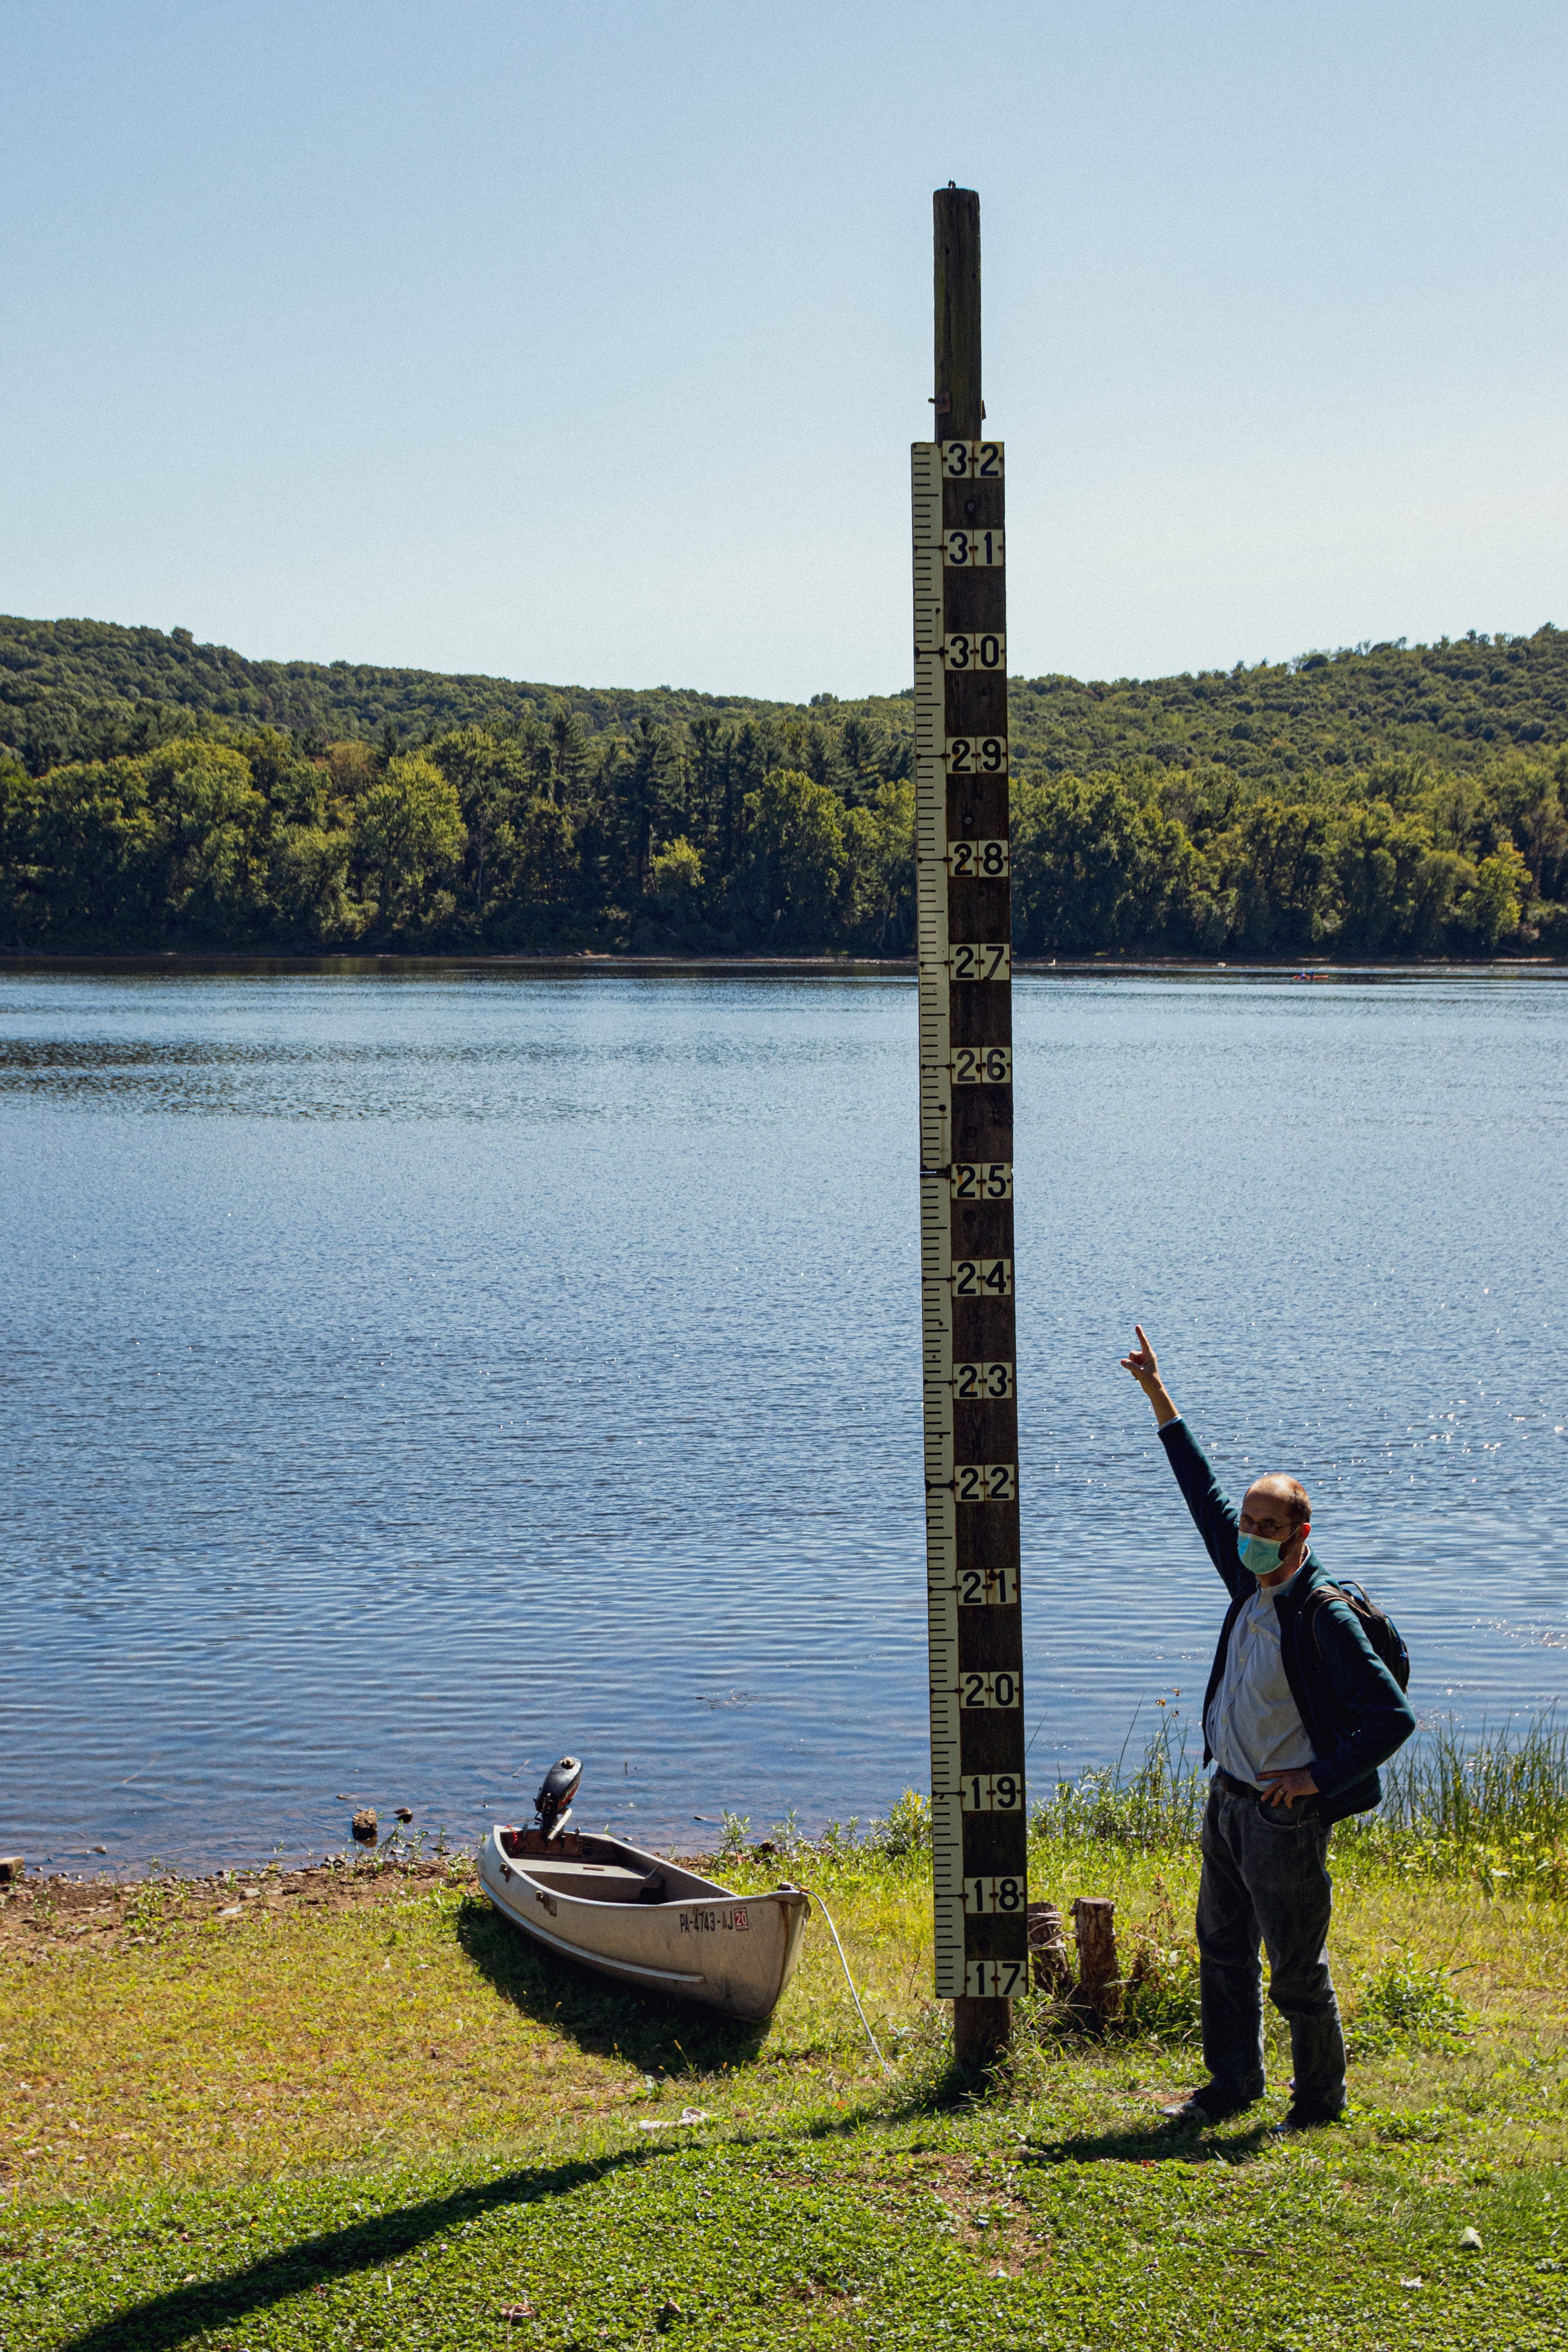
\includegraphics{selinsgrove.jpg}

\includegraphics{slides_files/mediabag/1280px-Harvey_2017-0.png}

\includegraphics{slides_files/mediabag/2023-12-02.jpg}
\end{frame}

\begin{frame}{Some things I've learned about you}
\phantomsection\label{some-things-ive-learned-about-you}
\begin{enumerate}[<+->]
\tightlist
\item
  You come from \ldots{}
\item
  You're taking this class because\ldots{}
\item
  You're interested in learning about CEVE or already planning to major
\item
  Interested in sustainable business
\end{enumerate}
\end{frame}

\section{About CEVE}\label{about-ceve}

\begin{frame}{What problems have Civil and Environmental Engineers
Solved?}
\phantomsection\label{what-problems-have-civil-and-environmental-engineers-solved}
In small groups:

\begin{enumerate}
\tightlist
\item
  Discuss this question
\item
  Have one person fill in group answers at TODO
\end{enumerate}
\end{frame}

\begin{frame}{}
\phantomsection\label{section}
\includegraphics[width=\textwidth,height=7.29167in]{slides_files/mediabag/Roman_aqueduct,_Sego.jpg}
\end{frame}

\begin{frame}{}
\phantomsection\label{section-1}
\includegraphics[width=\textwidth,height=7.29167in]{cholera.jpg}

\href{https://education.nationalgeographic.org/resource/mapping-a-london-epidemic/}{National
Geographic}
\end{frame}

\begin{frame}{}
\phantomsection\label{section-2}
\includegraphics[width=\textwidth,height=7.29167in]{slides_files/mediabag/2560px-Chase_Center_.jpg}
\end{frame}

\begin{frame}{}
\phantomsection\label{section-3}
\includegraphics[width=\textwidth,height=7.29167in]{slides_files/mediabag/2880px-Q_Bridge_in_N.jpg}
\end{frame}

\begin{frame}{Why aren't we ``done''?}
\phantomsection\label{why-arent-we-done}
In small groups:

\begin{enumerate}
\tightlist
\item
  Discuss this question
\item
  Have one person fill in group answers at TODO
\end{enumerate}
\end{frame}

\begin{frame}
\includegraphics[width=\textwidth,height=7.29167in]{slides_files/mediabag/2024-billion-dollar-.png}
\end{frame}

\begin{frame}
\includegraphics[width=\textwidth,height=7.29167in]{slides_files/mediabag/dby0crkfspr31.jpg}
\end{frame}

\begin{frame}
\includegraphics[width=\textwidth,height=7.29167in]{slides_files/mediabag/2021-Grades-Chart.jpg}
\end{frame}

\begin{frame}
\includegraphics[width=\textwidth,height=7.29167in]{slides_files/mediabag/6-Temperature.jpg}
\end{frame}

\begin{frame}
\includegraphics[width=\textwidth,height=7.29167in]{slides_files/mediabag/2560px-Toxic_Algae_B.jpg}
\end{frame}

\begin{frame}
\includegraphics[width=\textwidth,height=7.29167in]{slides_files/mediabag/2021-08-15T020705Z_1.jpg}
\end{frame}

\begin{frame}
\includegraphics[width=\textwidth,height=7.29167in]{outside-they-built.png}
\end{frame}

\section{About CEVE 101}\label{about-ceve-101}

\begin{frame}{Course Overview}
\phantomsection\label{course-overview}
\begin{enumerate}
\tightlist
\item
  Explore the intersection of built, information, and natural
  environments
\item
  Develop quantitative toolkit to understand \textbf{and improve}
  sustainability, resilience, and equity in infrastructure systems
\item
  Develop skills in data analysis, system modeling, and engineering
  design
\end{enumerate}
\end{frame}

\begin{frame}{Course Structure}
\phantomsection\label{course-structure}
\begin{enumerate}
\tightlist
\item
  Technical lectures
\item
  Topical seminars on applications
\item
  Team-based projects
\end{enumerate}
\end{frame}

\begin{frame}{Modules}
\phantomsection\label{modules}
Four modules, each culminating in a group design project

\begin{enumerate}
\tightlist
\item
  Climate and energy
\item
  Mobility and networks
\item
  Water and health
\item
  Coastal resilience
\end{enumerate}
\end{frame}

\begin{frame}{Learning Objectives}
\phantomsection\label{learning-objectives}
By the end of this course, you will be able to:

\begin{enumerate}
\tightlist
\item
  Understand interconnections between CEVE subfields
\item
  Apply fundamental principles to solve engineering problems
\item
  Generate high-quality engineering calculations and reports
\item
  Collaborate effectively in project teams
\item
  Recognize the impact of CEVE in addressing global challenges
\item
  Evaluate ethical implications of engineering decisions
\end{enumerate}
\end{frame}

\begin{frame}{Course Materials}
\phantomsection\label{course-materials}
\begin{enumerate}
\tightlist
\item
  No required textbook
\item
  All materials posted on course website or Canvas
\item
  Scientific papers accessible through Rice library
\item
  Recommended: Use Zotero for reference management
\end{enumerate}
\end{frame}

\begin{frame}{Grading}
\phantomsection\label{grading}
\begin{columns}[T]
\begin{column}{0.5\textwidth}
\textbf{Participation (40\%)}

\begin{enumerate}
\tightlist
\item
  In-class attendance
\item
  Assigned readings
\item
  Class discussions
\item
  Reading quizzes
\end{enumerate}
\end{column}

\begin{column}{0.5\textwidth}
\textbf{Projects (60\%)}

\begin{enumerate}
\tightlist
\item
  Four group design projects
\item
  One per module
\item
  Peer evaluations included
\end{enumerate}
\end{column}
\end{columns}
\end{frame}

\begin{frame}{Academic Integrity}
\phantomsection\label{academic-integrity}
\begin{enumerate}
\tightlist
\item
  Rice Honor Code applies
\item
  Collaboration encouraged, but work must represent your own
  understanding
\item
  Proper citation of sources required
\item
  Ask if you're unsure!
\end{enumerate}
\end{frame}

\begin{frame}{AI/ML Resource Policy}
\phantomsection\label{aiml-resource-policy}
\begin{enumerate}
\tightlist
\item
  LLMs (e.g., GPT) permitted with restrictions
\item
  Can be used for coding assistance
\item
  Not allowed for generating text submissions
\item
  You are responsible for understanding and verifying all output
\end{enumerate}
\end{frame}

\begin{frame}{Getting Help}
\phantomsection\label{getting-help}
\begin{enumerate}
\tightlist
\item
  Canvas Discussions for content questions
\item
  Office hours (sign up online!)
\item
  Email for personal matters
\end{enumerate}
\end{frame}

\begin{frame}{Course website}
\phantomsection\label{course-website}
\begin{itemize}
\tightlist
\item
  \url{https://jdossgollin.github.io/f24-ceve-101}
\item
  \href{https://jdossgollin.github.io/f24-ceve-101/syllabus.html}{Syllabus}
\item
  \href{https://jdossgollin.github.io/f24-ceve-101/lectures.html}{Lectures}
\end{itemize}
\end{frame}

\begin{frame}[fragile]{These slides}
\phantomsection\label{these-slides}
These slides use RevealJS and are made with Quarto. To print slides:

\begin{enumerate}
\tightlist
\item
  Open in Chrome / Brave
\item
  Press \texttt{e} to open print mode
\item
  Print using browser
\end{enumerate}
\end{frame}

\begin{frame}{See you Thursday!}
\phantomsection\label{see-you-thursday}
\end{frame}



\end{document}
